\documentclass[tikz,border=0cm,dvipsnames,x11names,rgb]{standalone}

\usepackage{amsmath,amssymb,amsfonts}
\usetikzlibrary{calc,
fit,
shapes.misc,
shapes.geometric,
arrows.meta,
fadings,
matrix,
chains,
scopes,
positioning}

\usepackage{pgfplots}
\usepackage{pgfplotstable}
\pgfplotsset{compat=1.18}



\usepackage[]{fontspec}

\setmainfont{Latin Modern Roman}
\setmonofont{Latin Modern Math}
\renewcommand{\textsc}[1]{{\fontfamily{lmr}\selectfont \scshape #1}}

\usepackage[]{bm}

\makeatletter
\@ifundefined{fromRoot}{\newcommand{\fromRoot}[1]{../../#1}}{}

\def\input@path{{../..}{..}{.}{./svg}{./pgfplots}{./tikzpicture}}
%or: \def\input@path{{/path/to/folder/}{/path/to/other/folder/}}
\makeatother

\newcommand*{\gf}[1]{\acrshort{gf}($#1$)}%
\newcommand*{\mpn}[1]{\bm{P}_{#1}}%
\newcommand*{\pn}[1]{%
  \ifthenelse{\equal{#1}{}}{$\mpn{0}$}{$\mpn{#1}$}%
}%

\newcommand*{\pk}[3]{%
  \ifthenelse{\equal{#1}{#2}}{\textcolor{red}{\phantom{.}$p_0$\phantom{.}}}{\phantom{.}$p_#3$\phantom{.}}%
}%


\newcommand*{\placeholder}{
\includegraphics[width=\linewidth, height=.25\textheight, keepaspectratio = true]{figures/certified_xilinx.png}}%

\newcommand*{\snr}{\acrshort{snr}}%
\newcommand*{\snrs}{\acrshortpl{snr}}%

\newcommand*{\mpd}[0]{p_\Delta}%
\newcommand*{\mpo}[0]{p_\omega}%
\newcommand*{\pd}[0]{$\mpd$}%
\newcommand*{\po}[0]{$\mpo$}%
\newcommand*{\mpfa}[0]{\mathcal{P}_{fa}}%
\newcommand*{\mpmd}[0]{\mathcal{P}_{md}}%
\newcommand*{\pfa}[0]{\acrshort{pfa}}%
\newcommand*{\pmd}[0]{\acrshort{pmd}}%
\newcommand*{\mnorm}[1]{\mathcal{L}_{#1}}%
\newcommand*{\norm}[1]{$\mnorm{#1}$}%
\newcommand*{\fft}{\acrshort{fft}}%
\newcommand*{\mfft}[1]{\mathcal{F}(#1)}%
\newcommand*{\mifft}[1]{\mathcal{F}^{-1}(#1)}%
\newcommand*{\ts}{\acrshort{ts}}%

\newcommand*{\cpp}[1]{C\textrm{++#1}}%
\newcommand*{\na}{\textrm{\textcolor{SlateGray4}{N/A}}}%

\newcommand*{\vect}[1]{\bm{#1}}%
\newcommand*{\mat}[1]{\bm{\mathrm{#1}}}%

\newcommand*{\task}[1]{\mathcal{T}_{#1}}%

\newcommand*{\sdr}{\acrshort{sdr}}%
\newcommand*{\fpga}{\acrshort{fpga}}%



\begin{document}

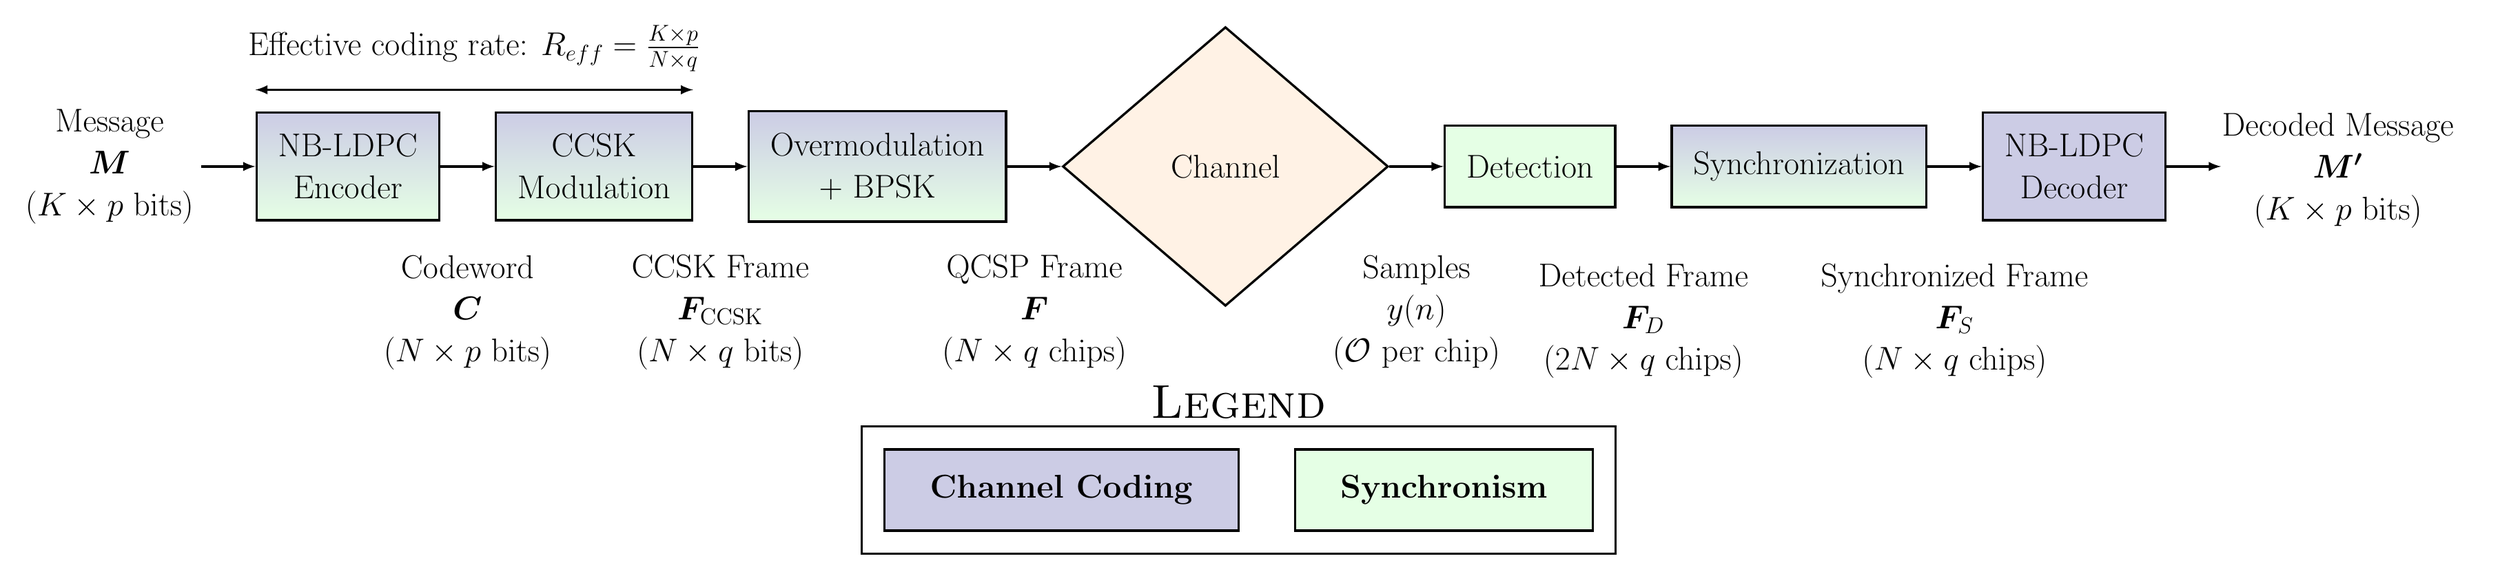
\begin{tikzpicture} [-latex,
    >=latex,
    auto,
    very thick,
    every node/.style={font=\LARGE},
    main node/.style={rectangle, draw,
        align = center, inner sep = 4mm}]

  \node [
    align=center,
    minimum height = 1.5cm
  ] (m) at (0, 0) {Message\\$\vect{M}$\\($K \times p$ bits)};

  \node [main node,
    top color = NavyBlue!20,
    bottom color = green!10,
    align=center,
    % minimum height = 1.5cm,
    right = 1cm of m
  ] (nbenc) {NB-LDPC\\Encoder};

  \node [main node,
    top color = NavyBlue!20,
    bottom color = green!10,
    % minimum height = 1.5cm,
    %minimum width = 3cm,
    right = 1cm of nbenc
  ] (ccskm) {CCSK\\Modulation};

  \node [main node,
    top color = NavyBlue!20,
    bottom color = green!10,
    % minimum height = 1.5cm,
    %minimum width = 3cm,
    right = 1cm of ccskm
  ] (bpskm) {Overmodulation\\$+$ BPSK};

  \node [diamond,
    draw,
    fill = orange!10,
    aspect = .5,
    minimum width = 6cm,
    right = 1 cm of bpskm
  ] (chan) {Channel};

  \node [main node,
    fill = green!10,
    minimum height = 1.5cm,
    %minimum width = 3cm,
    right = 1 cm of chan
  ] (ccskd)  {Detection};

  \node [main node,
    top color = NavyBlue!20,
    bottom color = green!10,
    minimum height = 1.5cm,
    %minimum width = 3cm,
    right = 1 cm of ccskd
  ] (ccsks) {Synchronization};

  \node [main node,
    fill = NavyBlue!20,
    % bottom color = NavyBlue!30,
    minimum height = 1.5cm,
    right = 1cm of ccsks
  ] (nbdec) {NB-LDPC\\Decoder};

  \node [align=center,
    right = .5 cm of nbdec] (mp) {\phantom{É}Decoded Message\phantom{É}\\$\vect{M'}$\\($K \times p$ bits)};

  \node [main node,
    fill = NavyBlue!20,
    minimum height = 1.5cm,
    % anchor = east,
    %  minimum width = 4cm,
    below = 5.2 cm of chan.west,
  ] (legchncod) {\phantom{O}\textbf{Channel Coding}\phantom{O}};

  \node [main node,
    fill = green!10,
    minimum height = 1.5cm,
    %  minimum width = 4cm,
    right = 1 cm of legchncod,
  ] (legmet) {\phantom{O}\textbf{Synchronism}\phantom{O}};

  \node [main node,
    fill=none,
    fit = (legchncod) (legmet),
    inner sep = 4mm,
    label = \textsc{\Huge Legend},
  ] (legend) {};

  %%%%%%%%%%%%%%%%%%%%%%%%%%%%%%

  \draw (m.east) -> (nbenc.west);

  \draw (nbenc.east) -> (ccskm.west)
  node [midway, align=center, below = 1.5 cm] {Codeword\\$\vect{C}$\\($N \times p$ bits)};

  \draw (ccskm.east) -> (bpskm.west)
  node [midway, align=center, below = 1.5 cm] {CCSK Frame\\$\vect{F}_{\mathrm{CCSK}}$\\($N \times q$ bits)};

    \draw (bpskm.east) -> (chan.west)
    node [midway, align=center, below = 1.5 cm] {QCSP Frame\\$\vect{F}$\\($N \times q$ chips)};

    \draw (chan.east) -> (ccskd.west)
    node [midway, align=center, below = 1.5 cm] {Samples\\$y(n)$\\($\mathcal{O}$ per chip)};

    \draw (ccskd.east) -> (ccsks.west)
    node [midway, align=center, below = 1.5 cm] {\phantom{É}Detected Frame\phantom{É}\\$\vect{F}_D$\\($2 N \times q$ chips)};

    \draw (ccsks.east) -> (nbdec.west)
    node [midway, align=center, below = 1.5 cm] {\phantom{É}Synchronized Frame\phantom{É}\\$\vect{F}_S$\\($N \times q$ chips)};

    \draw (nbdec.east) -> ($(mp.west) + (.5, 0)$);

  \draw [latex-latex] ($(0, .4) + (nbenc.north west)$) -- ($(0, .4) + (ccskm.north east)$)
  node [midway, align=center, above = .2cm] (Mp) {Effective coding rate: $R_{eff} = \frac{K \times p}{N \times q}$};
\end{tikzpicture}


\end{document}
